%!TEX root=/home/ska124/Dropbox/Thesis/thes-full.tex
%% Copyright 1998 Pepe Kubon
%%
%% `one.tex' --- 1st chapter for thes-full.tex, thes-short-tex from
%%                the `csthesis' bundle

%%%%%%%%%%%%%%%%%%%%%%%%%%%%%%%%%%%%%%%%%%%%%%%%%
%
%       Chapter 1 
%
%%%%%%%%%%%%%%%%%%%%%%%%%%%%%%%%%%%%%%%%%%%%%%%%

\chapter{Introduction}
\label{introduction}

Memory systems are an integral part of computer architecture whose overall design and organisation have remained unchanged since their inception. Early mainframe computers in the 1960's were known to use a hierarchial memory organisation. The memory technologies include semi-conductor, magnetic core, drum and disc. Caching would be used to fetch data and instructions into the fastest memory ahead of CPU accesses. Initally, accessing memory was only slightly slower than register access however as the difference grew, the need to mitigate the delay incurred for a memory access became extremely important. The rate at which computations were performed kept increasing however the rate at which data was fed to the processor from the memory system did not grow at the same rate. In order to alleviate the effects of slow memory, smaller faster memory was built close to the processor to cache frquently used data. The first documented use of a data cache was in the IBM System/360 Model 85\cite{liptay68}. Now multilevel memory hierarchies are used which are composed of fast static random access memory and slower dynamic random access memory before going to disk.


\section{Cache Memory Systems}

Long story about cache memory systems and how they are organised
Diagrams of standard caches

\section{Motivation for Change}

In traditional caches, the cache block defines the fundamental unit of
data movement and space allocation in caches. The blocks in the data
array are uniformly sized to simplify the insertion/removal of blocks,
simplify cache refill requests, and support low complexity tag
organization. Unfortunately, conventional caches are inflexible (fixed
block granularity and fixed \# of blocks) and caching efficiency is
poor for applications that lack high spatial locality.  Cache blocks
influence multiple system metrics including bandwidth, miss rate, and
cache utilization. The block granularity plays a key role in
exploiting spatial locality by effectively prefetching neighboring
words all at once. However, the neighboring words could go unused due
to the low lifespan of a cache block. The unused words occupy
interconnect bandwidth and pollute the cache, which increases the \#
of misses. We evaluate the influence of a fixed
granularity block below.

\subsection{Cache Utilization}

In the absence of spatial locality, multi-word cache blocks (typically 64
bytes on existing processors) tend to increase cache pollution and fill the
cache with words unlikely to be used.  To quantify this pollution, we segment
the cache line into words (8 bytes) and track the words touched before the
block is evicted.  We define utilization as the average \# of words touched in
a cache block before it is evicted. We study a comprehensive collection of
workloads from a variety of domains: 6 from PARSEC~\cite{Bienia:2008:PBS:1454115.1454128}, 7 from
SPEC2006, 2 from SPEC2000, 3 Java workloads from DaCapo~\cite{Blackburn:2006:DBJ:1167473.1167488}, 3
commercial workloads (Apache, SpecJBB2005, and TPC-C~\cite{Llanos:2006:TOT:1228268.1228270}), and the
Firefox web browser.  Subsets within benchmark suites were chosen based on
demonstrated miss rates on the fixed granularity cache (i.e., whose working
sets did not fit in the cache size evaluated) and with a spread and diversity
in cache utilization.  We classify the benchmarks into 3 groups
based on the utilization they exhibit: Low ($<$33\%), Moderate (33\%---66\%),
and High (66\%+) utilization (see Table~\ref{table:benchmark_categories}).

\begin{table}[!htb]
\vspace{-10pt}
\begin{center}
\caption{Benchmark Groups}
\label{table:benchmark_categories}
{
  \begin{tabular}{ |@{~}c@{~}|@{~}c@{~}|@{~}p{0.6\columnwidth}@{~}|}
    \hline
    Group & Utilization \% & Benchmarks \\
    \hline
    Low        & 0 --- 33\% & art, soplex, twolf, mcf, canneal, lbm, omnetpp \\
    \hline
    Moderate   & 34 --- 66\% & astar, h2, jbb, apache, x264, firefox, tpc-c, freqmine, fluidanimate \\
    \hline
    High       & 67 --- 100\% & tradesoap, facesim, eclipse, cactus, milc, ferret \\
    \hline
  \end{tabular}
 }
\end{center}
\end{table}


\begin{figure}[!h]

 \begin{center}
  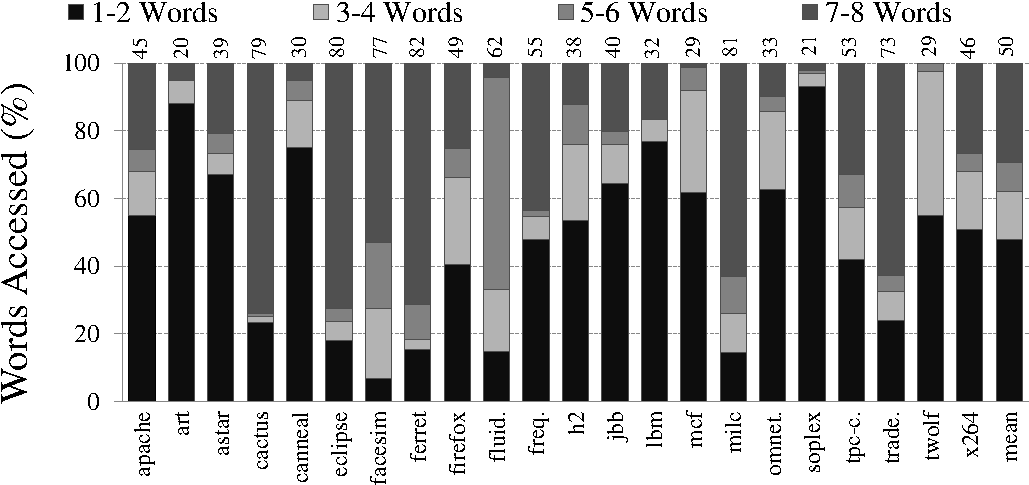
\includegraphics[width=0.5\textwidth]{files/Plots/05-StackBar_Word_Access_64K.pdf}
  \caption{Distribution of words touched in a cache
    block. Avg. utilization is on top. (Config:
    64K, 4 way, 64-byte block.)}
  \label{fig:stackbar_words_64k}
 \end{center}

\end{figure}

Figure~\ref{fig:stackbar_words_64k} shows the histogram of words
touched at the time of eviction in a cache line of a 64K, 4-way cache 
(64-byte block, 8 words per block) across the different benchmarks. 
Seven applications have
less than 33\% utilization and 12 of them are dominated (>50\%) by 1-2
word accesses.  In applications with good spatial locality (cactus,
ferret, tradesoap, milc, eclipse) more than 50\% of the evicted blocks have
7-8 words touched. Despite similar average utilization for
applications such as astar and h2 (39\%), their distributions
are dissimilar; $\simeq$70\% of the blocks in astar have 1-2 words
accessed at the time of eviction, 
whereas $\simeq$50\% of the blocks in h2 have 1-2 words accessed per block.  
Utilization for a single application also changes over time; for example, ferret's 
average utilization, measured as the average fraction of words used in 
evicted cache lines over 50 million instruction windows, 
varies from 50\% to 95\% with a periodicity of roughly 400 million instructions.   
%Different temporal phases and 
%memory regions
%within an application may have different requirements: in firefox, 40\% of
%the blocks have 1--2 words touched, 26\% of the blocks have 3--4 words
%touched, and 34\% have 5+ words touched. 
%Overall, the utilization plot
%indicates the need for run time adjustment of cache block granularity.


\subsection{Effect of Block Granularity on Miss Rate and Bandwidth}

Cache miss rate directly correlates with performance, while under
current and future wire-limited technologies, bandwidth
directly correlates with dynamic energy.
Figure~\ref{fig:scatter_bw_64k_1m} shows the influence of block
granularity on miss rate and bandwidth for a 64K L1 cache and a 1M L2
cache keeping the number of ways constant. For the 64K L1, the plots
highlight the pitfalls of simply decreasing the block size to
accommodate the Low group of applications; miss rate increases by
2$\times$ for the High group when the block size is changed from 64B
to 32B; it increases by 30\% for the Moderate group. A smaller block
size decreases bandwidth proportionately but increases miss rate. With
a 1M L2 cache, the lifetime of the cache lines increases significantly, 
improving overall utilization. Increasing the block size from
64$\to$256 halves the miss rate for all application groups. 
The bandwidth is increased by 2$\times$ for the Low and Moderate.

% SK- Apache 3x miss rate drop not observed anymore. Occured due to
% different length warmup for Oracle and Fixed runs.

Since miss rate and bandwidth have different optimal block
granularities, we use the following metric: $\frac{1}{Miss Rate \times
  Bandwidth}$ to determine a fixed block granularity suited to an
application that takes both criteria into account.
Table~\ref{table:bwmr_classify} shows the block size that maximizes
the metric for each application.  It can be seen that different
applications have different block granularity requirements.  For
example, the metric is maximized for apache at 128 bytes and for
firefox (similar utilization) at 32 bytes.  Furthermore, the optimal
block sizes vary with the cache size as the cache lifespan
changes. This highlights the challenge of picking a single block size
at design time especially when the working set does not fit in the
cache.
%In short, \textit{the tradeoff between increasing the 
%  cache block granularity to achieve spatial prefetching and lower miss rate, 
%  and reducing the granularity to minimize traffic and pollution needs
%  adaptive cache blocks.}

\subsection{Need for adaptive cache blocks}
Our observations motivate the need for adaptive cache line
granularities that match the spatial locality of the data access patterns
in an application. In summary:
\begin{itemize}
  \item  Smaller cache lines improve utilization but tend to increase
    miss rate and potentially traffic for applications with good
    spatial locality, affecting the overall performance.
  \item Large cache lines pollute the cache space and interconnect
    with unused words for applications with poor spatial locality, 
   significantly decreasing the caching efficiency.
\item Many applications waste a significant fraction of the cache
  space. Spatial locality varies not only across applications but also
  within each application, for different data structures as well as 
  different phases of access over time.   
%\item Optimizing miss rate (impacts performance), bandwidth (impacts
%  dynamic energy), and utilization simultaneously with a fixed size
%  cache line is not tractable, since in many cases the optimality is
%  achieved at different block sizes.
\end{itemize}


\begin{figure}[!t]

  \subfloat[64K - Low]{
    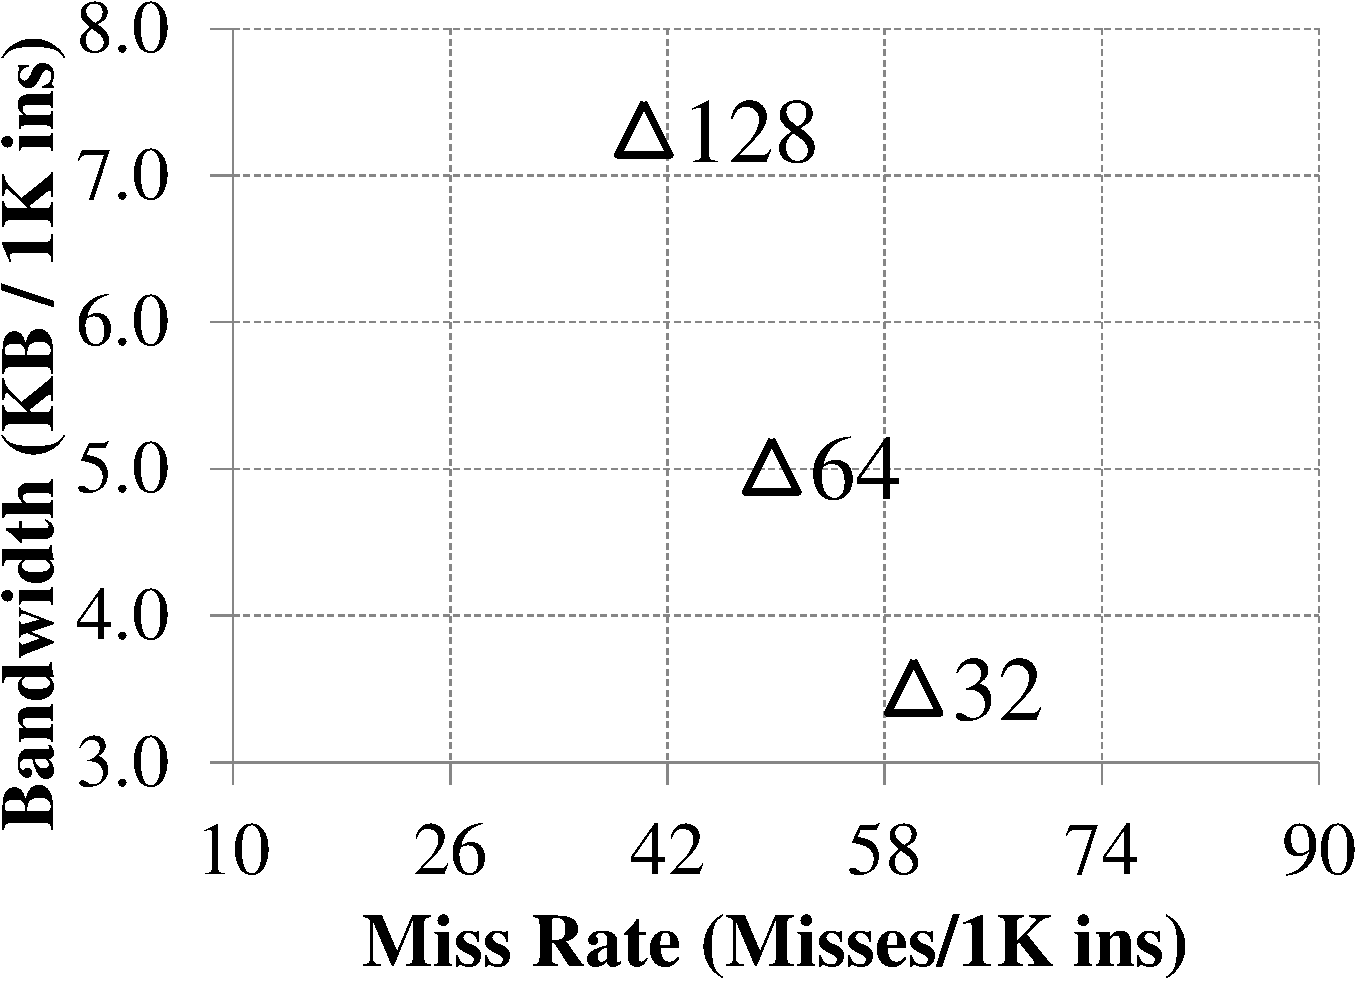
\includegraphics[width=0.24\textwidth]{files/Plots/05-Scatter_Bw_Miss_64K_low.pdf}
  }
  \subfloat[1M - Low]{
     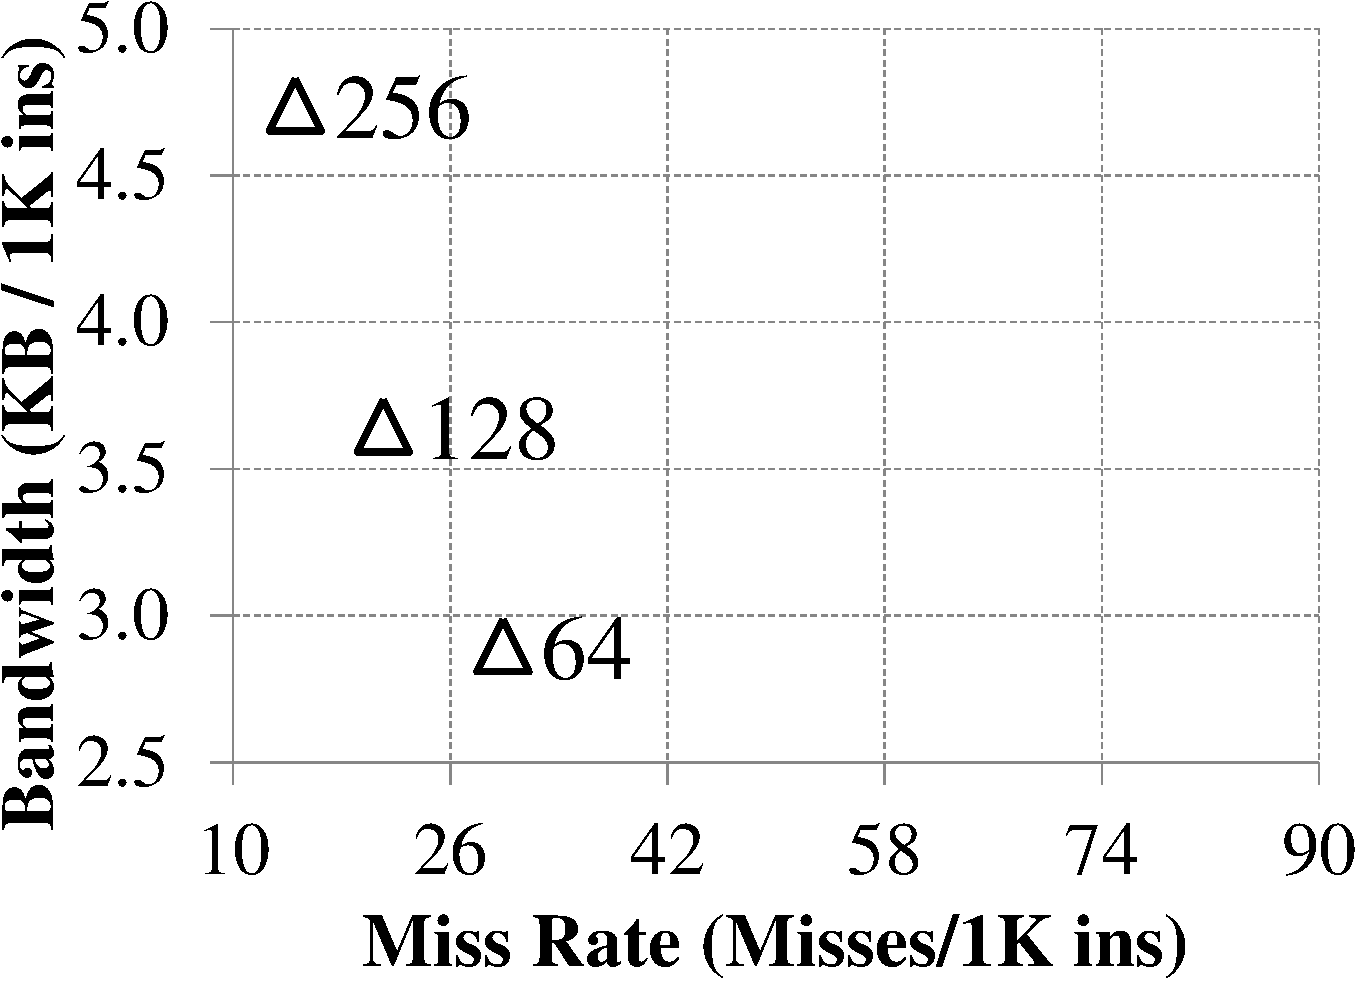
\includegraphics[width=0.24\textwidth]{files/Plots/05-Scatter_Bw_Miss_1M_low.pdf}
  }
  
  \subfloat[64K - Moderate]{
    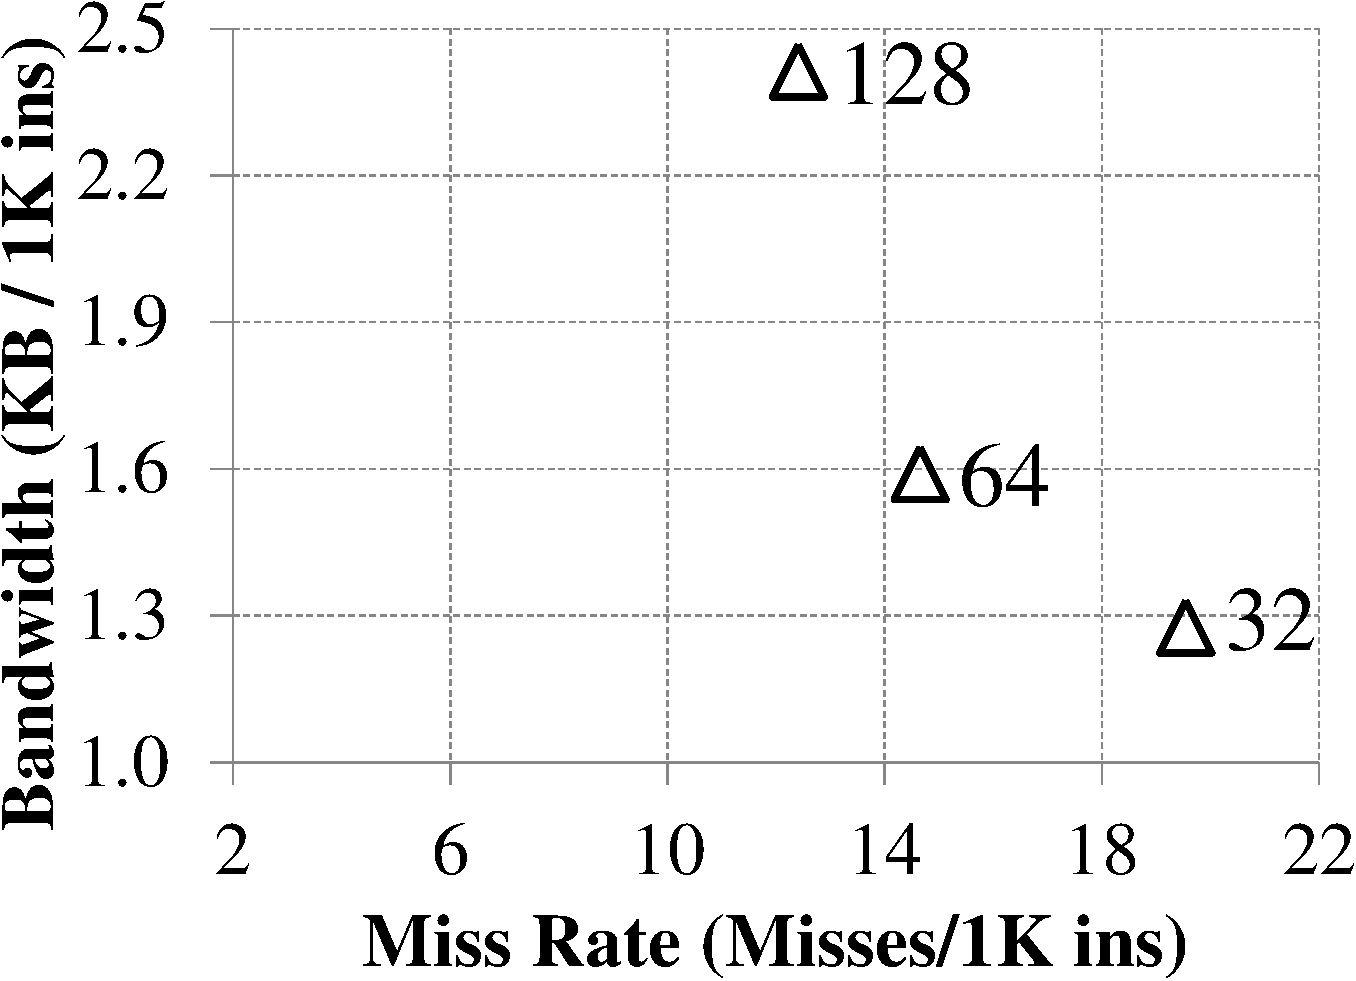
\includegraphics[width=0.24\textwidth]{files/Plots/05-Scatter_Bw_Miss_64K_mod.pdf}
  }
  \subfloat[1M - Moderate]{
     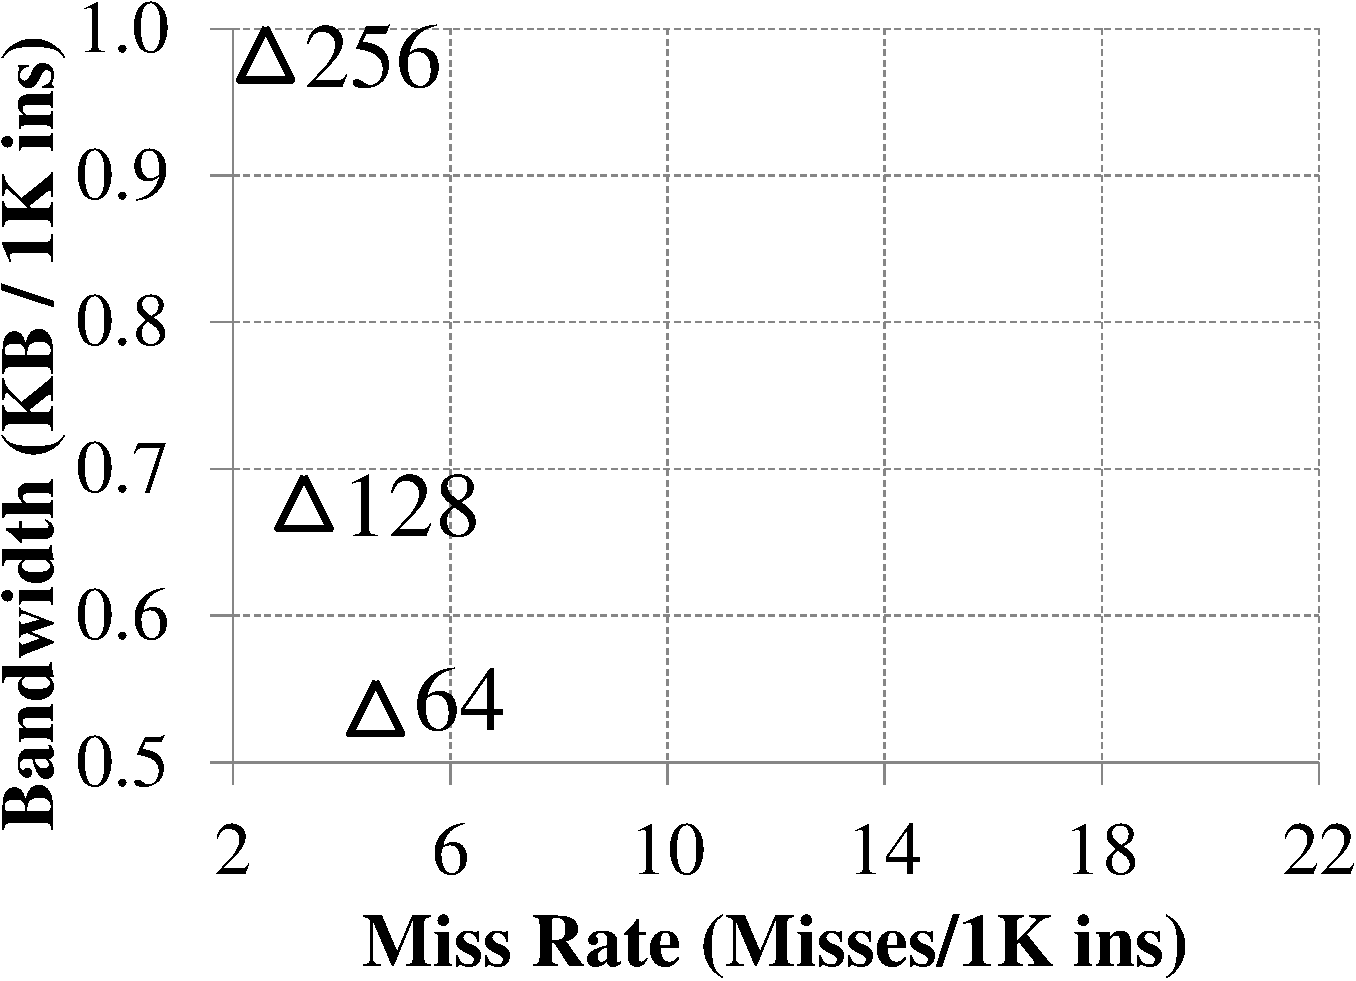
\includegraphics[width=0.24\textwidth]{files/Plots/05-Scatter_Bw_Miss_1M_mod.pdf}
  }
    
  \subfloat[64K - High]{
    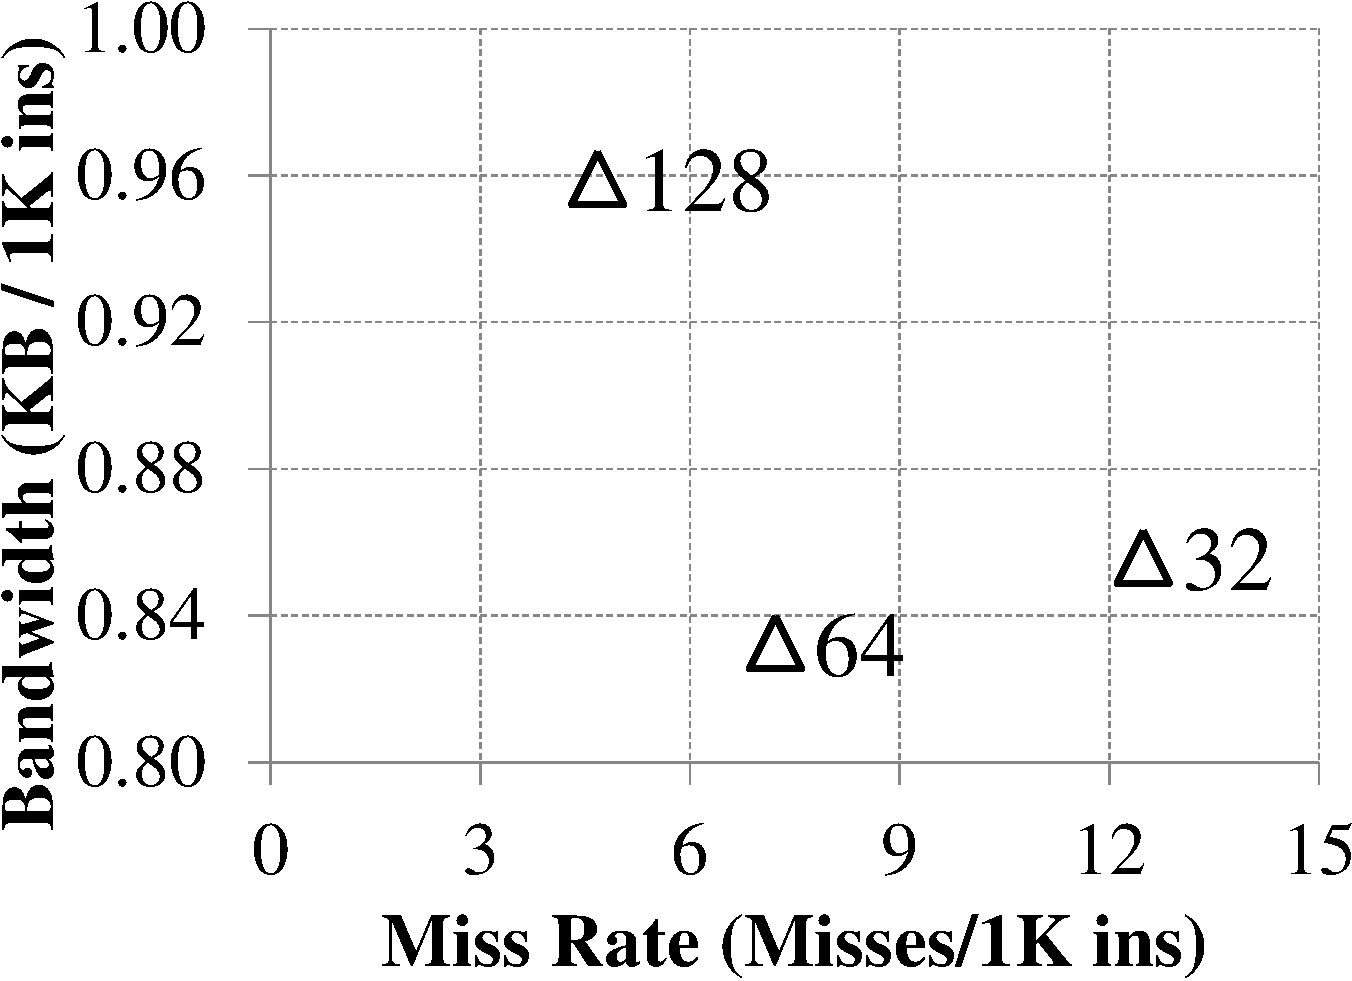
\includegraphics[width=0.24\textwidth]{files/Plots/05-Scatter_Bw_Miss_64K_high.pdf}
  }
  \subfloat[1M - High]{
     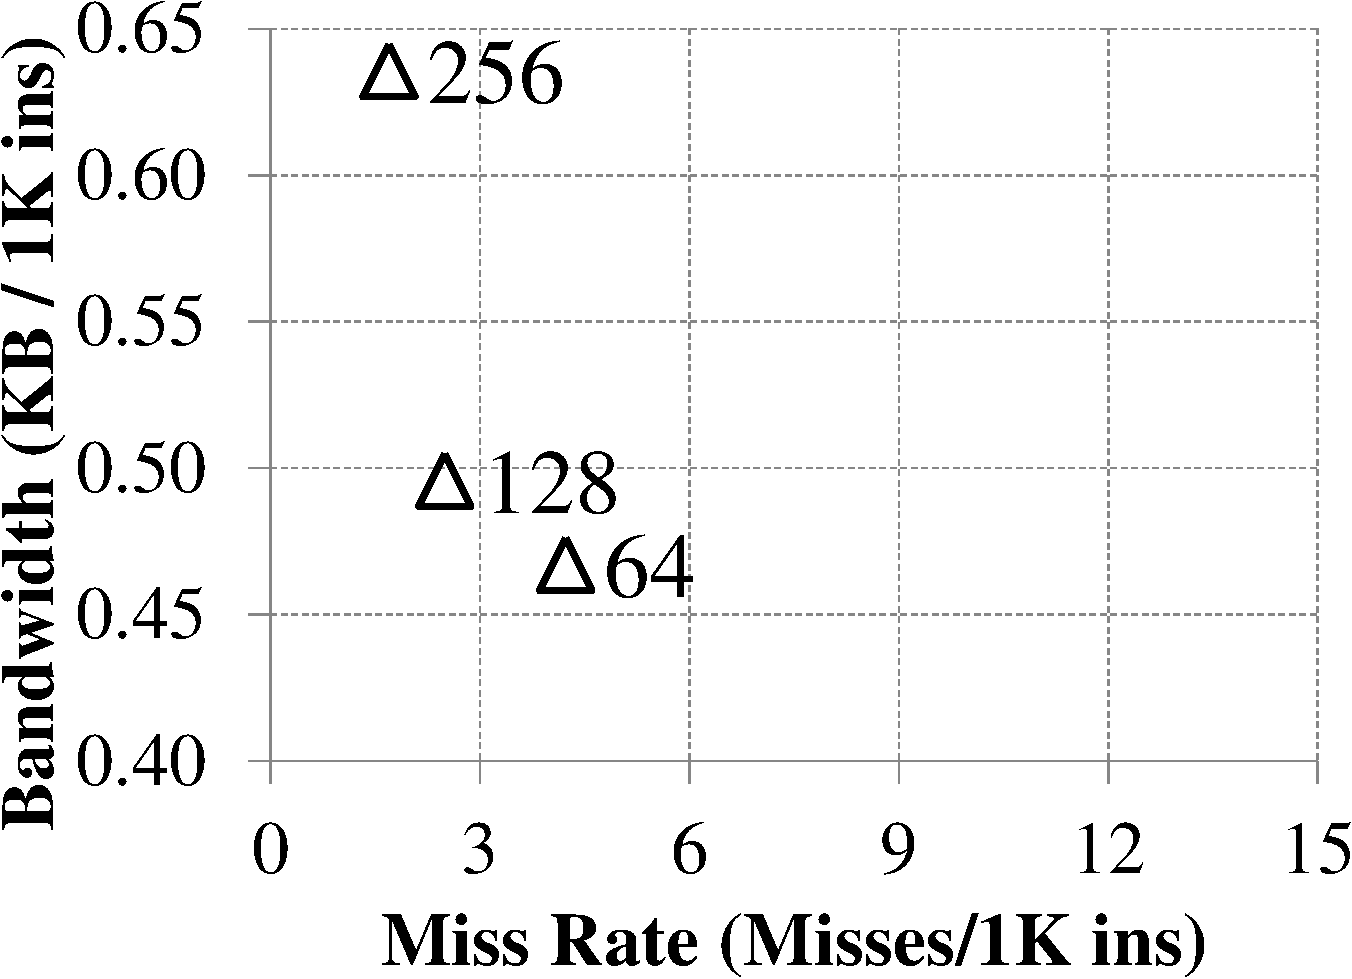
\includegraphics[width=0.24\textwidth]{files/Plots/05-Scatter_Bw_Miss_1M_high.pdf}
  }

  \caption{Bandwidth vs. Miss Rate. (a),(c),(e): 64K, 4-way
    L1. (b),(d),(f): 1M, 8-way LLC.  Markers on the plot indicate cache
    block size. Note the different scales for different groups.}
  \label{fig:scatter_bw_64k_1m}
  \end{figure}


\begin{table}[!h]
\caption{Optimal block size. Metric: $\mathbf{\frac{1}{Miss-rate \times Bandwidth}}$}
\label{table:bwmr_classify}
\begin{center}
{
\small
  \begin{tabular}{ |@{~}c@{~}| m{0.72\columnwidth} |}
    \hline
    \multicolumn{2}{|c|}{64K, 4-way} \\
    \hline
    Block  & Benchmarks \\
    \hline
    32B   & cactus, eclipse, facesim, ferret, firefox, fluidanimate,freqmine, milc, tpc-c, tradesoap \\
    \hline
    64B   &  art \\
    \hline
    128B  & apache, astar, canneal, h2, jbb, lbm, mcf, omnetpp, soplex, twolf, x264 \\
    \hline
    \multicolumn{2}{|c|}{1M, 8-way} \\
    \hline
    Block & Benchmarks \\
    \hline
    64B  & apache, astar, cactus, eclipse, facesim, ferret, firefox, freqmine, h2, lbm, milc, omnetpp, tradesoap, x264\\
    \hline
    128B & art\\
    \hline
    256B  & canneal, fluidanimate, jbb, mcf, soplex, tpc-c, twolf\\
    \hline
  \end{tabular}
}
\end{center}
\end{table}




\section{Dissertation Outline}